
\documentclass[fleqn,a4paper,12pt]{article}

% fleqn to left align equations
%\setlength{\textwidth}{2in}
\usepackage{hyperref}
\usepackage{fancyhdr}
\usepackage{enumitem}
%\renewcommand{\familydefault}{\rmdefault}
\renewcommand{\familydefault}{\sfdefault}
%\usepackage{helvet}
%\pagestyle{fancy}
\date{}
%\pagenumbering{gobble}
\usepackage{geometry}
\pagenumbering{gobble}
\usepackage{multicol}
\usepackage{tikz}
\usepackage{amsmath}
\usepackage{amsfonts}
\usepackage{mathtools,xparse}

%\fancyhf{}
%\pagestyle{fancy}
%\rhead{Mina Jafari}
%\lhead{ML-HW1}
\newcommand{\norm}[1]{\left\lVert#1\right\rVert}

%Abernethy
\newcounter{probnum}
\newcounter{subprobnum}
\newcounter{subsubprobnum}
\stepcounter{probnum}
\stepcounter{subprobnum}
\stepcounter{subsubprobnum}

\newcommand{\nsubprob}[2]{\addtolength{\leftskip}{-3em}\vspace{0em} \noindent \textbf{ \noindent #1) \stepcounter{subprobnum}} #2\par \addtolength{\leftskip}{3em}}

\def \probmargin{1.2em}
\def \probvspace{0em}

\newcommand{\nprob}[2]
{
	
	\vspace{\probvspace}
	\setcounter{subprobnum}{1}
	\setlength{\leftskip}{0em}
	\noindent \arabic{probnum}) \textbf{#1. } #2 
	\vspace{\probvspace}
	\stepcounter{probnum}
}

\newcommand{\subprob}[1]
{
	
	\setlength{\leftskip}{\probmargin}
	\setcounter{subsubprobnum}{1}
	
	\def \subttl{\textbf{(\alph{subprobnum}) }}
	\settowidth{\parindent}{\subttl}
	\addtolength{\leftskip}{\parindent}
	\setlength{\parindent}{-\parindent}
	\subttl #1
	\stepcounter{subprobnum}
	\vspace{\probvspace}
	\setlength{\parindent}{0em}
	
}

\newcommand{\subsubprob}[1]
{
	
	\setlength{\leftskip}{\probmargin}
	\addtolength{\leftskip}{\probmargin}
	
	\def \subttl{\textbf{(\roman{subsubprobnum}) }}
	\settowidth{\parindent}{\subttl}
	\addtolength{\leftskip}{\parindent}
	\setlength{\parindent}{-\parindent}
	\subttl #1
	\stepcounter{subsubprobnum}
	\vspace{\probvspace}
	\setlength{\parindent}{0em}
	
}
%end-abernethy

\geometry{a4paper,left=20mm,right=20mm,top=20mm,bottom=20mm}
%\renewcommand{\headrulewidth}{1.5 pt}

\hypersetup
{
    pdfauthor={Mina Jafari},
    pdfsubject={Homework1},
    pdftitle={MachineLearning},
    pdfkeywords={ML-HW1}
}
\linespread{1.3}

\makeatletter
\def \TVname{Jacob Abernethy}
\newcommand{\hwclass}[1]{\def \TVclass{#1}}
\newcommand{\hwdue}[1]{\def \TVdue{#1}}
\newcommand{\hwassignment}[1]{\def \TVassignment{#1}}
\makeatother

% Title Heading
\renewcommand{\maketitle}
{
	\begin{center}
		\newlength{\titlerulewidth}
		\def \hmwkttl{{\TVclass\, - \TVassignment}}
		\settowidth{\titlerulewidth}{\hmwkttl}
		
		\rule{\titlerulewidth}{1pt}\\[3mm]
		\hmwkttl \\[3mm]
	%	\makebox[\titlerulewidth]{\small \TVname \hspace{1em} \hfill \hfill  group member: Joshua Kammeraad} \\
		\makebox[\titlerulewidth]{\small \TVname \hspace{1em}} \\
		\makebox[\titlerulewidth]{\footnotesize {group member: Joshua Kammeraad} \hspace{1em}} \\
		\rule{\titlerulewidth}{1pt}\\[3mm]
	\end{center}
	
	\vspace{3em}
}

\def\TVname{Mina Jafari}

\hwclass{EECS 545 -- Machine Learning}
\hwdue{11:00pm 01/25/2016}
\hwassignment{Homework \#1}
\begin{document}
\maketitle	

\nprob{Question 1}{

\subprob{}{

\subsubprob{}{ True.
	
	$(A^{-1})^{\top} = (A^{\top})^{-1}$
	
	multiply both sides by $((A^{\top})^{-1})^{-1}$ and we know $((A^{\top})^{-1})^{-1} = A^{\top}$
	
	$A^{\top} (A^{-1})^{\top} = A^{\top} (A^{\top})^{-1}$
	
	$A^{\top} (A^{-1})^{\top} = I$
	
	$(A^{-1} A)^{\top} = I$
	
	$I^{\top} = I$

	$I = I$
}
\subsubprob{}{ False.
	
$	A = \begin{bmatrix}
		3 & 1 \\
		7 & 3 \\
		\end{bmatrix}$ , 
$	B = \begin{bmatrix}
		1 & -5 \\
		12 & 27 \\
		\end{bmatrix}$
		
$(A+B)^{-1} = \begin{bmatrix}
			  0.15306122 & 0.02040816 \\
			 -0.09693878 & 0.02040816 \\
			  \end{bmatrix}$
			 
$A^{-1} + B^{-1} = \begin{bmatrix}
					1.81034483 & -0.44252874\\
					-3.63793103 & 1.51149425\\
				   \end{bmatrix}$
}
		
\subsubprob{}{ True.
	
	If $A$ is symmetric, $A = A^{\top}$. Prove $A^{-1} = (A^{-1})^{\top}$.
	
	$A A^{-1} = I$
	
	$(AA^{-1})^{\top} = I^{\top} = I$
	
	$(A^{-1})^{\top} A^{\top} = I$ and $A^{\top} = A$
	
	$(A^{-1})^{\top} A = I$
	
	$(A^{-1})^{\top} A A^{-1} = I A^{-1}$
	
	$(A^{-1})^{\top} = A^{-1}$
}
}	
	
\subprob{}{

	$XX^{\top} = (U\Sigma V^{\top})(U\Sigma V^{\top})^{\top} = U\Sigma V^{\top}V\Sigma^{\top}U^{\top} = U\Sigma\Sigma^{\top}U^{\top}$
	
	$XX^{\top} = Q\Lambda Q^{-1}$
	
	$\implies U\Sigma\Sigma^{\top}U^{\top} =  Q\Lambda Q^{-1}$
	
	$\implies Q=U, Q^{-1} = U^{\top}, \Lambda = \Sigma \Sigma^{\top}$
	
	The eigen decomposition results in eigenvalues $\lambda _i = \Lambda_{ii} = \sigma_i^{2}$ for $1 \leq i \leq m$ (for non-zero diagonal elements of $\Lambda$) and columns of $U$ are orthonormal and constitute the eigenvectors of $XX^{\top}$.
}

\subprob{}{
	\subsubprob{}{

	757.00219118, 158.20556896, 130.31529335
	}
	\subsubprob{}{
\begin{equation*}
		\lVert{A-B}\rVert_F^{2} = 68125.6048172
\end{equation*}
	
	\begin{figure}[!ht]
	\centering
	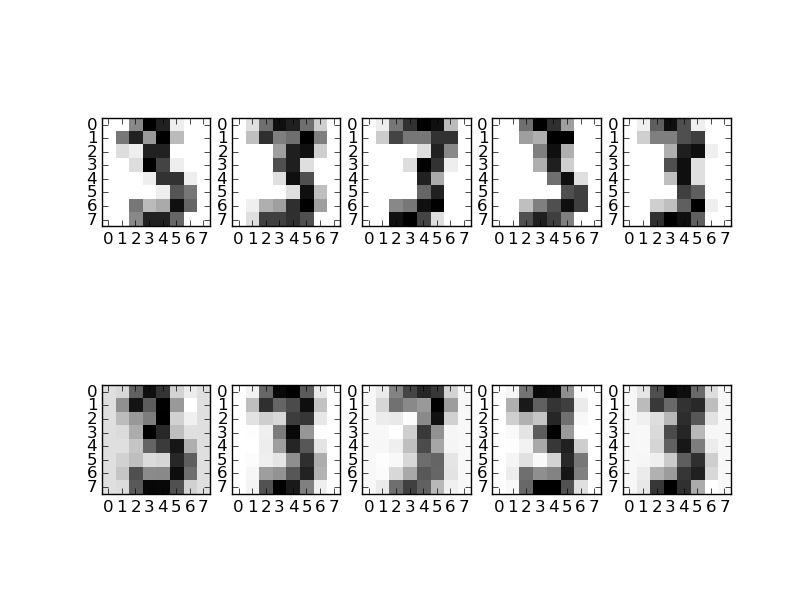
\includegraphics[width=0.7\textwidth]{figure_1.png}
	\end{figure}
	}
}
}

\vspace{20cm}

\nprob{Question 2}{
	\subprob{}{
		\subsubprob{}{ depends. 
	
	If H \& D are \textbf{independent}, then $\frac{P(H)P(D)}{P(D)}$ ? $P(H)$, so $P(H=h|D=d) = P(H=h)$.
	}

	\subsubprob{}{$\geq$
	
	$P(H=h|D=d) = \frac{P(H \cap D)}{P(D)}$
	
	$P(D=d|H=h)P(H=h) = \frac{P(D \cap H)}{P(H)}P(H)$
	
	$\frac{P(H \cap D)}{P(D)}$ ? $P(D \cap H)$
	
	$\frac{P(D \cap H)}{P(D)}$ ? $P(D \cap H)$
	
	So, $P(H=h|D=d) \geq P(D=d|H=h)P(H=h)$
	}
	}

\subprob{}{
	\subsubprob{}{
		
	\begin{flalign*}
	\mathbb{E}[X] = \int_{x}p(x)Xdx    
	\end{flalign*}
	\begin{flalign*}
	\hspace{10.5mm} \mathbb{E}_Y[\mathbb{E}_X[X|Y]] &= \int_{y}p(y) \int_{x}p(x|y)Xdxdy = \int_{y}\int_{x}p(y) \frac{p(x,y)}{p(y)} Xdxdy & \\ 
									&= \int_{x}\int_{y}p(x,y)Xdxdy = \int_{x}p(x)Xdx \\
	\end{flalign*}
	$\implies \mathbb{E}[X] = \mathbb{E}_Y[\mathbb{E}_X[X|Y]]$
	}
	\subsubprob{}{
	
	$\text{var}[X] = \mathbb{E}[X^2] - (\mathbb{E}[X])^2$
	
	
	$\mathbb{E}_Y[\text{var}_X[X|Y]] + \text{var}_Y[\mathbb{E}_X[X|Y]] = \\
	\mathbb{E}_Y[\mathbb{E}_X[X^2|Y] - (\mathbb{E}_X[X|Y])^2 ] + \mathbb{E}_Y[(\mathbb{E}_X[X|Y])^2] - (\mathbb{E}_Y[(\mathbb{E}_X[X|Y])])^2 \\
	\mathbb{E}_Y[\mathbb{E}_X[X^2|Y]] - \mathbb{E}_Y[(\mathbb{E}_X[X|Y])^2] + \mathbb{E}_Y[(\mathbb{E}_X[X|Y])^2] - (\mathbb{E}_Y[(\mathbb{E}_X[X|Y])])^2$
	
	middle terms cancel out and based on part \textbf{i} of the question:
	
	$\mathbb{E}_Y[\mathbb{E}_X[X^2|Y]] - (\mathbb{E}_Y[(\mathbb{E}_X[X|Y])])^2 = \mathbb{E}[X^2] - (\mathbb{E}[X])^2 = \text{var}[X]$

	}
	}
}
\vspace{8cm}
\nprob{Question 3}{
	\subprob{}{
		\textbf{Prove that if $A$ is PSD, then $\lambda_i \geq 0$:}
		
		Assume $A$ is PSD, then $x^{\top}Ax \geq 0$.
		
		Since $A$ is real and symmetric, we can use the spectral theorem to express $A$ as $A = U\Lambda U^{\top}$ and $Au_i = \lambda_iu_i$ for all $i$.
		
		If $x^{\top}Ax \geq 0$ is true for any vector $x$, then it should be true for the eigenvectors of $A$, $u_i$ for all $i$.
		
		We can write $u_i^{\top}Au_i \geq 0$ based on  $x^{\top}Ax \geq 0$.
		
		$u_i^{\top}Au_i \geq 0 \rightarrow u_i^{\top}\lambda_i u_i \geq 0 \rightarrow \lambda_i u_i^{\top}u_i \geq 0 \xrightarrow[]{\lVert u_i \rVert = \sqrt{u_i^{\top}u_i}} \lambda_i\lVert u_i \rVert^2 \geq 0$ 
		
		Since $\lVert u_i \rVert > 0 \implies \lambda_i \geq 0$
		
		\textbf{Prove that if $\lambda_i \geq 0$, then $A$ is PSD:}
		
		Assume $\lambda_i \geq 0$. The spectral theorem holds since $A$ is real and symmetric, then $A = U\Lambda U^{\top}$ and $Au_i = \lambda_iu_i$ for all $i$.
		
		$Au_i = \lambda_iu_i \rightarrow u_i^{\top}Au_i = u_i^{\top} \lambda_iu_i \rightarrow u_i^{\top}Au_i = \lambda_i u_i^{\top} u_i = \lambda_i$
		
		If $\lambda_i \geq 0 \implies u_i^{\top}Au_i \geq 0$ for $1 \leq i \leq d$
		
		$A$ is a real and symmetric $d \times d$ matrix. $U$ is an orthogonal $d \times d$ matrix and its columns are eigenvectors of the $A$, so it spans the whole space of $A$. Since vectors $u_i$ and $x$ span the same space, we can write $u_i^{\top}Au_i \geq 0$ into the general form of $x^{\top}Ax \geq 0$. This property means $A$ is PSD ($A \geq 0$).
	}
	\subprob{}{
		\textbf{Prove that if $A$ is PD, then $\lambda_i > 0$:}
		
		Assume $A$ is PD, then $x^{\top}Ax > 0$ for all $x \neq 0$.
		
		Since $A$ is real and symmetric, we can use the spectral theorem to express $A$ as $A = U\Lambda U^{\top}$ and $Au_i = \lambda_iu_i$ for all $i$.
		
		If $x^{\top}Ax > 0$ is true for any vector $x$, then it should be true for the eigenvectors of $A$, $u_i$ for all $i$.
		
		We can write $u_i^{\top}Au_i > 0$ based on  $x^{\top}Ax > 0$.
		
		$u_i^{\top}Au_i > 0 \rightarrow u_i^{\top}\lambda_i u_i > 0 \rightarrow \lambda_i u_i^{\top}u_i > 0 \xrightarrow[]{\lVert u_i \rVert = \sqrt{u_i^{\top}u_i}} \lambda_i\lVert u_i \rVert^2 > 0$ 
		
		Since $\lVert u_i \rVert > 0 \implies \lambda_i > 0$
		
		\textbf{Prove that if $\lambda_i > 0$, then $A$ is PD:}
		
		Assume $\lambda_i > 0$. The spectral theorem holds since $A$ is real and symmetric, then $A = U\Lambda U^{\top}$ and $Au_i = \lambda_iu_i$ for all $i$.
		
		$Au_i = \lambda_iu_i \rightarrow u_i^{\top}Au_i = u_i^{\top} \lambda_iu_i \rightarrow u_i^{\top}Au_i = \lambda_i u_i^{\top} u_i = \lambda_i$
		
		If $\lambda_i > 0 \implies u_i^{\top}Au_i > 0$ for $1 \leq i \leq d$
		
		$A$ is a real and symmetric $d \times d$ matrix. $U$ is an orthogonal $d \times d$ matrix and its columns are eigenvectors of the $A$, so it spans the whole space of $A$. Since vectors $u_i$ and $x$ span the same space, we can write $u_i^{\top}Au_i > 0$ into the general form of $x^{\top}Ax > 0$. This property means $A$ is PD ($A > 0$).
	}
	}

\vspace{30cm}
\nprob{Question 4}{
	\begin{flalign*}
	f(x_i;\lambda) = \frac{\lambda^{x_i} e^{-\lambda}}{x_i!}
	\end{flalign*}
	\begin{flalign*}
	\sum_{i=1}^{n} \log{\frac{\lambda^{x_i} e^{-\lambda}}{x_i!}}
	\end{flalign*}
	\begin{flalign*}
	\sum_{i=1}^{n} (\log{\lambda^{x_i}} - \lambda - \log{x_i!})
	\end{flalign*}
	\begin{flalign*}
	\frac{df(x_i;\lambda)}{d\lambda} = \sum_{i=1}^{n}(\frac{x_i}{\lambda}-1) = 0
	\end{flalign*}
	\begin{flalign*}
	\frac{1}{\lambda} \sum_{i=1}^{n}(x_i - n) = 0
	\end{flalign*}
	\begin{flalign*}
	\lambda = \frac{\sum_{i=1}^{n} x_i}{n}
	\end{flalign*}
	}
	
\vspace{20cm}	
\nprob{Question 5}{
	\subprob{}{
		Strictly convex means $f(\frac{x+y}{2}) < \frac{f(x)}{2} + \frac{f(y)}{2}$. 
		
		For a given point $z$ which minimizes the function $f(x)$, $f(z) < f(x \neq z)$.
		
		If the function $f(x)$ has more than one global minimizer ($z$), then exits a point $l$ in which $f(z) = f(l)$:
		
		$f(\frac{z+l}{2}) < \frac{f(z)}{2} + \frac{f(l)}{2} \rightarrow  f(\frac{z+l}{2}) < \frac{f(z)}{2} + \frac{f(z)}{2} \rightarrow  f(\frac{z+l}{2}) < f(z)$ 
		
		There is a point $\frac{z+l}{2}$ such that $f(\frac{z+l}{2}) < f(z)$. So, $z$ is not the global minimizer and $f(x)$ cannot have more than one global minimizer.
	}
	
	\subprob{}{
		\begin{flalign*}
		f(\mathbf{x}) = f(\mathbf{y}) + \langle \bigtriangledown f(\mathbf{y}), \mathbf{x}-\mathbf{y} \rangle + \frac{1}{2} \langle \mathbf{x}-\mathbf{y}, \bigtriangledown^2
		f(\mathbf{y})(\mathbf{x}-\mathbf{y}) \rangle + o(\|\mathbf{x}-\mathbf{y}\|^2)
		\end{flalign*}
		\begin{flalign*}
		f(\mathbf{x}) = f(\mathbf{x^*}) + \langle \bigtriangledown f(\mathbf{x^*}), \mathbf{x}-\mathbf{x^*} \rangle + \frac{1}{2} \langle \mathbf{x}-\mathbf{x^*}, \bigtriangledown^2
		f(\mathbf{x^*})(\mathbf{x}-\mathbf{x^*}) \rangle + o(\|\mathbf{x}-\mathbf{x^*}\|^2)
		\end{flalign*}
		\begin{flalign*}
		\bigtriangledown f(\mathbf{x^*}) = 0 \implies f(\mathbf{x}) = f(\mathbf{x^*}) + \frac{1}{2} \langle \mathbf{x}-\mathbf{x^*}, \bigtriangledown^2
		f(\mathbf{x^*})(\mathbf{x}-\mathbf{x^*}) \rangle + o(\|\mathbf{x}-\mathbf{x^*}\|^2)
		\end{flalign*}
		\begin{flalign*}
		f(\mathbf{x}) - f(\mathbf{x^*}) = \frac{1}{2} \langle \mathbf{x}-\mathbf{x^*}, \bigtriangledown^2
		f(\mathbf{x^*})(\mathbf{x}-\mathbf{x^*}) \rangle + o(\|\mathbf{x}-\mathbf{x^*}\|^2)
		\end{flalign*}
		There exists a radius $r$ such that $\|x-x^*\| \leq r \implies f(\mathbf{x}) - f(\mathbf{x^*}) \geq 0$ since $x^*$ is a local minimizer in that radius.
		\begin{flalign*}
		\frac{1}{2} \langle \mathbf{x}-\mathbf{x^*}, \bigtriangledown^2
		f(\mathbf{x^*})(\mathbf{x}-\mathbf{x^*}) \rangle + o(\|\mathbf{x}-\mathbf{x^*}\|^2) \geq 0
		\end{flalign*}
		\begin{flalign*}
		\frac{1}{2} \langle \norm{\mathbf{x}-\mathbf{x^*}} \frac{\mathbf{x}-\mathbf{x^*}}{\norm{\mathbf{x}-\mathbf{x^*}}}, \bigtriangledown^2
		f(\mathbf{x^*})(\norm{\mathbf{x}-\mathbf{x^*}} \frac{\mathbf{x}-\mathbf{x^*}}{\norm{\mathbf{x}-\mathbf{x^*}}}) \rangle + o(\|\mathbf{x}-\mathbf{x^*}\|^2) \geq 0
		\end{flalign*}
		\begin{flalign*}
		\frac{1}{2} \norm{\mathbf{x}-\mathbf{x^*}}^2 \langle \frac{\mathbf{x}-\mathbf{x^*}}{\norm{\mathbf{x}-\mathbf{x^*}}}, \bigtriangledown^2
		f(\mathbf{x^*})(\frac{\mathbf{x}-\mathbf{x^*}}{\norm{\mathbf{x}-\mathbf{x^*}}}) \rangle + o(\|\mathbf{x}-\mathbf{x^*}\|^2) \geq 0
		\end{flalign*}
		\begin{flalign*}
		\frac{\mathbf{x}-\mathbf{x^*}}{\norm{\mathbf{x}-\mathbf{x^*}}} \hspace{0.5cm}\text{and}\hspace{0.5cm} \bigtriangledown^2
		f(\mathbf{x^*}) \hspace{0.5cm}\text{are constant in a given direction} \implies
		\end{flalign*}
		\begin{flalign*}
		c = \frac{1}{2} \langle \frac{\mathbf{x}-\mathbf{x^*}}{\norm{\mathbf{x}-\mathbf{x^*}}}, \bigtriangledown^2
		f(\mathbf{x^*})(\frac{\mathbf{x}-\mathbf{x^*}}{\norm{\mathbf{x}-\mathbf{x^*}}}) \rangle ,\hspace{0.5 cm} t = \|\mathbf{x}-\mathbf{x^*}\|^2 \hspace{0.5 cm}\text{and}
		\end{flalign*}
		\begin{flalign*}
		\lim_{t \to 0} \frac{o(t)}{ct} = 0 \implies o(t) \hspace{0.2cm}\text{goes to zero faster than}\hspace{0.2cm} ct \implies
		\end{flalign*}
		\begin{flalign*}
		\frac{1}{2} \norm{\mathbf{x}-\mathbf{x^*}}^2 \langle \frac{\mathbf{x}-\mathbf{x^*}}{\norm{\mathbf{x}-\mathbf{x^*}}}, \bigtriangledown^2
		f(\mathbf{x^*})(\frac{\mathbf{x}-\mathbf{x^*}}{\norm{\mathbf{x}-\mathbf{x^*}}}) \rangle > o(\|\mathbf{x}-\mathbf{x^*}\|^2) \implies
		\end{flalign*}
		\begin{flalign*}
		\text{if  }
		\frac{1}{2} \norm{\mathbf{x}-\mathbf{x^*}}^2 \langle \frac{\mathbf{x}-\mathbf{x^*}}{\norm{\mathbf{x}-\mathbf{x^*}}}, \bigtriangledown^2
		f(\mathbf{x^*})(\frac{\mathbf{x}-\mathbf{x^*}}{\norm{\mathbf{x}-\mathbf{x^*}}}) \rangle + o(\|\mathbf{x}-\mathbf{x^*}\|^2) \geq 0 \implies
		\end{flalign*}
		\begin{flalign*}
				\frac{1}{2} \norm{\mathbf{x}-\mathbf{x^*}}^2 \langle \frac{\mathbf{x}-\mathbf{x^*}}{\norm{\mathbf{x}-\mathbf{x^*}}}, \bigtriangledown^2
				f(\mathbf{x^*})(\frac{\mathbf{x}-\mathbf{x^*}}{\norm{\mathbf{x}-\mathbf{x^*}}}) \rangle \geq 0 \implies
		\end{flalign*}
		\begin{flalign*}
		\langle \mathbf{x}-\mathbf{x^*}, \bigtriangledown^2
		f(\mathbf{x^*})(\mathbf{x}-\mathbf{x^*}) \rangle \geq 0
		\implies  (\mathbf{x}-\mathbf{x^*})^{\top} \bigtriangledown^2
		f(\mathbf{x^*})(\mathbf{x}-\mathbf{x^*}) \geq 0
		\implies \bigtriangledown^2 f(\mathbf{x^*}) \geq 0
		\end{flalign*}
	}
	
	\subprob{}{
		Show if $f(\mathbf{x})$ is convex, then $\mathbf{x^{\top}}\bigtriangledown^2 f(\mathbf{y})\mathbf{x} \geq 0$ for all $\mathbf{y} \in \mathbb{R}^d$.
		\begin{flalign*}
		f(\mathbf{x}) = f(\mathbf{y}) + \langle \bigtriangledown f(\mathbf{y}), \mathbf{x}-\mathbf{y} \rangle + \frac{1}{2} \langle \mathbf{x}-\mathbf{y}, \bigtriangledown^2
		f(\mathbf{y})(\mathbf{x}-\mathbf{y}) \rangle + o(\|\mathbf{x}-\mathbf{y}\|^2)
		\end{flalign*}
		A convex function satisfies $f(\mathbf{x}) \geq f(\mathbf{y}) + \bigtriangledown f(\mathbf{y}) \cdot (\mathbf{x}-\mathbf{y})$ for any $x, y$.
		\begin{flalign*}
		f(\mathbf{x}) \geq f(\mathbf{y}) + \langle \bigtriangledown f(\mathbf{y}), \mathbf{x}-\mathbf{y} \rangle \implies \\
		\frac{1}{2} \langle \mathbf{x}-\mathbf{y}, \bigtriangledown^2
		f(\mathbf{y})(\mathbf{x}-\mathbf{y}) \rangle + o(\|\mathbf{x}-\mathbf{y}\|^2) \geq 0
		\end{flalign*} 
		\begin{flalign*}
		\frac{1}{2} \langle \mathbf{x}-\mathbf{y}, \bigtriangledown^2
		f(\mathbf{y})(\mathbf{x}-\mathbf{y}) \rangle + o(\|\mathbf{x}-\mathbf{y}\|^2) \geq 0
		\end{flalign*}
		\begin{flalign*}
		\frac{1}{2} \langle \norm{\mathbf{x}-\mathbf{y}} \frac{\mathbf{x}-\mathbf{y}}{\norm{\mathbf{x}-\mathbf{y}}}, \bigtriangledown^2
		f(\mathbf{y})(\norm{\mathbf{x}-\mathbf{y}} \frac{\mathbf{x}-\mathbf{y}}{\norm{\mathbf{x}-\mathbf{y}}}) \rangle + o(\|\mathbf{x}-\mathbf{y}\|^2) \geq 0
		\end{flalign*}
		\begin{flalign*}
		\frac{1}{2} \norm{\mathbf{x}-\mathbf{y}}^2 \langle \frac{\mathbf{x}-\mathbf{y}}{\norm{\mathbf{x}-\mathbf{y}}}, \bigtriangledown^2
		f(\mathbf{y})(\frac{\mathbf{x}-\mathbf{y}}{\norm{\mathbf{x}-\mathbf{y}}}) \rangle + o(\|\mathbf{x}-\mathbf{y}\|^2) \geq 0
		\end{flalign*}
		\begin{flalign*}
		\frac{\mathbf{x}-\mathbf{y}}{\norm{\mathbf{x}-\mathbf{y}}} \hspace{0.2cm}\text{and}\hspace{0.2cm} \bigtriangledown^2
		f(\mathbf{y}) \hspace{0.2cm}\text{are constant in a given direction} \implies
		\end{flalign*}
		\begin{flalign*}
		c = \frac{1}{2} \langle \frac{\mathbf{x}-\mathbf{y}}{\norm{\mathbf{x}-\mathbf{y}}}, \bigtriangledown^2
		f(\mathbf{y})(\frac{\mathbf{x}-\mathbf{y}}{\norm{\mathbf{x}-\mathbf{y}}}) \rangle ,\hspace{0.5 cm} t = \|\mathbf{x}-\mathbf{y}\|^2 \hspace{0.5 cm}\text{and}
		\end{flalign*}
		\begin{flalign*}
		\lim_{t \to 0} \frac{o(t)}{ct} = 0 \implies o(t) \hspace{0.2cm}\text{goes to zero faster than}\hspace{0.2cm} ct \implies
		\end{flalign*}
		\begin{flalign*}
		\frac{1}{2} \norm{\mathbf{x}-\mathbf{y}}^2 \langle \frac{\mathbf{x}-\mathbf{y}}{\norm{\mathbf{x}-\mathbf{y}}}, \bigtriangledown^2
		f(\mathbf{y})(\frac{\mathbf{x}-\mathbf{y}}{\norm{\mathbf{x}-\mathbf{y}}}) \rangle > o(\|\mathbf{x}-\mathbf{y}\|^2) \implies
		\end{flalign*}
		\begin{flalign*}
		\text{if  }
		\frac{1}{2} \norm{\mathbf{x}-\mathbf{y}}^2 \langle \frac{\mathbf{x}-\mathbf{y}}{\norm{\mathbf{x}-\mathbf{y}}}, \bigtriangledown^2
		f(\mathbf{y})(\frac{\mathbf{x}-\mathbf{y}}{\norm{\mathbf{x}-\mathbf{y}}}) \rangle + o(\|\mathbf{x}-\mathbf{y}\|^2) \geq 0 \implies
		\end{flalign*}
		\begin{flalign*}
		\frac{1}{2} \norm{\mathbf{x}-\mathbf{y}}^2 \langle \frac{\mathbf{x}-\mathbf{y}}{\norm{\mathbf{x}-\mathbf{y}}}, \bigtriangledown^2
		f(\mathbf{y})(\frac{\mathbf{x}-\mathbf{y}}{\norm{\mathbf{x}-\mathbf{y}}}) \rangle \geq 0 \implies
		\end{flalign*}
		\begin{flalign*}
		\langle \mathbf{x}-\mathbf{y}, \bigtriangledown^2
		f(\mathbf{y})(\mathbf{x}-\mathbf{y}) \rangle \geq 0
		\implies  (\mathbf{x}-\mathbf{y})^{\top} \bigtriangledown^2
		f(\mathbf{y})(\mathbf{x}-\mathbf{y}) \geq 0
		\implies \bigtriangledown^2 f(\mathbf{y}) \geq 0
		\end{flalign*}
		
		\vspace{2cm}
		
		Show if $x^{\top}\bigtriangledown^2 f(\mathbf{x})x \geq 0$ for all $\mathbf{x,y} \in \mathbb{R}^d$, then $f(x)$ is convex.
		\begin{flalign*}
		f(\mathbf{x}) = f(\mathbf{y}) + \langle \bigtriangledown f(\mathbf{y}), \mathbf{x}-\mathbf{y} \rangle + \frac{1}{2} \langle \mathbf{x}-\mathbf{y}, \bigtriangledown^2 f(\mathbf{y} + t(\mathbf{x}-\mathbf{y}))(\mathbf{x}-\mathbf{y}) \rangle
		\end{flalign*}
		\begin{flalign*}
		f(\mathbf{x}) - f(\mathbf{y}) - \langle \bigtriangledown f(\mathbf{y}), \mathbf{x}-\mathbf{y} \rangle = \frac{1}{2} \langle \mathbf{x}-\mathbf{y}, \bigtriangledown^2 f(\mathbf{y} + t(\mathbf{x}-\mathbf{y}))(\mathbf{x}-\mathbf{y}) \rangle
		\end{flalign*}
		\begin{flalign*}
		\text{if  }x^{\top}\bigtriangledown^2 f(\mathbf{x})x \geq 0 \implies 
		\frac{1}{2} \langle \mathbf{x}-\mathbf{y}, \bigtriangledown^2 f(\mathbf{y} + t(\mathbf{x}-\mathbf{y}))(\mathbf{x}-\mathbf{y}) \rangle \geq 0 \text{  for  } t \in (0,1) \implies\\
		f(\mathbf{x}) - f(\mathbf{y}) - \langle \bigtriangledown f(\mathbf{y}), \mathbf{x}-\mathbf{y} \rangle \geq 0 \\
		f(\mathbf{x}) \geq f(\mathbf{y}) + \langle \bigtriangledown f(\mathbf{y}), \mathbf{x}-\mathbf{y} \rangle \\
		f(\mathbf{x}) \geq f(\mathbf{y}) + \bigtriangledown f(\mathbf{y}) \cdot (\mathbf{x}-\mathbf{y})
		\end{flalign*}
		This is the property of a convex function, so $f(x)$ is convex.
	}
	
	\subprob{}{
		\begin{flalign*}
		f(x) = \frac{1}{2} x^{\top}Ax + b^{\top}x + c
		\end{flalign*}
		\begin{flalign*}
		f''(x) = \frac{1}{2} (2A) = A
		\end{flalign*}
		
		if $y^{\top}Ay \geq 0$, $f(x)$ is convex for all $x \in \mathbb{R}^d$.
		
		if $y^{\top}Ay > 0$, $f(x)$ is strictly convex for all $x \in \mathbb{R}^d$.
	}
	}

\end{document}